\chapter{測定、密度行列、エントロピー}

二重スリット実験は、測定問題をその最も小さく有用な形で含んでいる。二つの選択肢がコヒーレントなままであれば、それらの振幅は干渉する。別の系が、どちらの選択肢が取られたかの記録を獲得すると、対象と記録者はもつれ合い、干渉は変化する。その機構を厳密なものにしてから、トレース、密度行列、エントロピー---もつれを定量化するために必要な言語を導入する。

\section{二重スリット実験の再構築}

位置\(0\)に源があり、二つの開口\(A\)と\(B\)があり、到達可能な位置が正規直交状態\(\{|m\rangle\}\)で表されるスクリーンがある離散模型を考える。粒子は電子でも光子でも、その他の任意の量子物体でもよい。これを電子と呼び、そのスピンを無視して、位置だけを議論の対象となる自由度とする。障壁の残りの部分は閉じている。すなわち、\(A\)または\(B\)以外の任意の位置に到達した電子は反射される。

構造上の原理は線形性である。二つの状態が
\begin{equation}
|A\rangle\longrightarrow |A'\rangle,
\qquad
|B\rangle\longrightarrow |B'\rangle,
\end{equation}
と発展するなら、任意の重ね合わせは同じ係数で発展する：
\begin{equation}
\alpha|A\rangle+\beta|B\rangle
\longrightarrow
\alpha|A'\rangle+\beta|B'\rangle.
\end{equation}

対称な配置では、源は二つの開口に等しい振幅で供給する。黒板でのように共通の規格化因子を省略すると、
\begin{equation}
|0\rangle\longrightarrow |A\rangle+|B\rangle.
\end{equation}
規格化された状態は\((|A\rangle+|B\rangle)/\sqrt{2}\)であろう。省略された因子は干渉の議論において何の役割も果たさない。

次に各経路を別々に調べる。開口からスクリーンへの伝播は
\begin{align}
|A\rangle &\longrightarrow \sum_m \psi_m|m\rangle, \\
|B\rangle &\longrightarrow \sum_m \phi_m|m\rangle.
\end{align}
の形をとる。複素数\(\psi_m\)は\(A\)から出発してスクリーン位置\(m\)に到達する振幅であり、\(\phi_m\)は\(B\)から出発した場合の対応する振幅である。

\begin{figure}[htbp]
\centering
\includegraphics[width=0.68\textwidth]{lecture_07_figure_02.png}
\caption{スクリーン基底における\(A\)経路と\(B\)経路の別々の展開。}
\lectureframe{00:05:39}
\end{figure}

\(B\)が閉じている場合、\(m\)における確率は
\begin{equation}
P_A(m)=|\psi_m|^2.
\end{equation}
である。\(A\)が閉じている場合、
\begin{equation}
P_B(m)=|\phi_m|^2.
\end{equation}
である。古典的確率論では、両方の開口が利用可能なときにこれら二つの答えを加えることを示唆するであろう。量子力学は代わりにまず振幅を加える：
\begin{equation}
|A\rangle+|B\rangle
\longrightarrow
\sum_m(\psi_m+\phi_m)|m\rangle.
\end{equation}
固定されたスクリーン位置では、
\begin{align}
P(m)
&=|\psi_m+\phi_m|^2 \\
&=|\psi_m|^2+|\phi_m|^2
  +\psi_m^*\phi_m+\phi_m^*\psi_m.
\end{align}

\begin{figure}[htbp]
\centering
\includegraphics[width=0.70\textwidth]{lecture_07_figure_03.png}
\caption{4項からなるスクリーン確率。最後の二つの項が干渉項である。}
\lectureframe{00:09:21}
\end{figure}

対称点では\(\psi_m=\phi_m\)であり、二つの選択肢は互いに強め合う。それらの位相が\(\pi\)だけ異なる点では\(\psi_m=-\phi_m\)であり、確率は消える。どちらか一方の経路だけでもその点に到達できるが、両方の経路を開くと電子がそこに到達するのを妨げうる。ここで疑問は避けられない：何かがどちらの開口が使われたかを記録すると、何が変わるのか？

\section{検出器がもつれ合う}

状態\(|u\rangle\)と\(|d\rangle\)をもつ補助的な二状態系を導入する。この模型ではこれは電子のスピンではない。最小限の外部装置である。初期状態で検出器はトリガーされていない：
\begin{equation}
|0,d\rangle.
\end{equation}
\(A\)を通る場合には検出器が反転し、\(B\)を通る場合には検出器が変化しないように相互作用を配置する：
\begin{equation}
|0,d\rangle
\longrightarrow
|A,u\rangle+|B,d\rangle.
\end{equation}
電子が開口を離れた後、それはもはや補助スピンと相互作用しない。したがって二つの分岐は
\begin{align}
|A,u\rangle &\longrightarrow \sum_m\psi_m|m,u\rangle, \\
|B,d\rangle &\longrightarrow \sum_m\phi_m|m,d\rangle,
\end{align}
として伝播し、最終状態は
\begin{equation}
|\Psi\rangle
=\sum_m\left(\psi_m|m,u\rangle+\phi_m|m,d\rangle\right).
\end{equation}
である。経路と検出器の記録は今やもつれ合っている。検出器を読めば、どちらの開口が使われたかが明らかになるであろう。

\begin{classroomqa}
\lecturetimestamp{00:13:24}
\audiencequestion{スピンが反転したとき、波束はすでに収縮しているのか？}
\lecturerresponse{電子だけについては、収縮という言葉を使ってもよい。経路の選択肢はもはや干渉しない。しかし、電子--検出器の完全な系については、どちらの分岐も捨て去られていない。状態は依然として\(|A,u\rangle+|B,d\rangle\)である。装置を含めることは、\emph{電子が収縮した}という記述を、系--装置のもつれ合いが確立されたという正確な記述に置き換える。}
\end{classroomqa}

補助スピンは単に便利なポインターにすぎない。発火したかしないかの装置、放出されたか存在しないかの光子、あるいはその他の任意の識別可能な記録の対が同じ役割を果たしうる。

\begin{classroomqa}
\lecturetimestamp{00:15:17}
\audiencequestion{金属板を通過すること自体が常に経路の記録を残すのか？}
\lecturerresponse{必ずしもそうではない。重要なのは、相互作用が板を識別可能な最終状態に残すかどうかである。板に励起ギャップがあり、電子がそれを励起するのに十分なエネルギーを持たないなら、持続的な内部の印を残す必要はない。単なる相互作用では十分ではない。二つの選択肢が識別可能な記録と相関しなければならない。}
\end{classroomqa}

\begin{classroomqa}
\lecturetimestamp{00:16:29}
\audiencequestion{板の反跳から、電子が上側と下側のどちらの開口を通ったかを明らかにできるだろうか。}
\lecturerresponse{逆向きの運動量のキックが、十分に区別可能な板の状態を生み出す場合に限られる。よく局在した板は、すでに広い運動量波動関数をもっている。小さな上向きと下向きのずれはほとんど完全に重なりうるため、反跳状態は直交せず、経路の記録を一義的に与えない。ここで不確定性原理が干渉を守っているのである。}
\end{classroomqa}

部分的な記録は可能である。検出器がわずかにキックされるだけなら、二つの最終的な記録状態は直交する必要はない。その場合、干渉は消えるのではなく減少する。形式的な計算では、まず完全測定の極限の場合を取る：
\begin{equation}
\langle u|d\rangle=0.
\end{equation}

\section{射影演算子による計算}

次に、検出器の結果を問わずに、電子が固定されたスクリーン位置\(m\)に到達する確率を計算する。合成ヒルベルト空間において、\emph{電子が\(m\)}にあるという性質は、次で張られる二次元部分空間である：
\begin{equation}
|m,u\rangle,\qquad |m,d\rangle.
\end{equation}
対応する射影演算子は
\begin{equation}
\Pi_m
=|m,u\rangle\langle m,u|
 +|m,d\rangle\langle m,d|.
\end{equation}

\begin{figure}[htbp]
\centering
\includegraphics[width=0.66\textwidth]{lecture_07_figure_04.png}
\caption{固定されたスクリーン位置への射影演算子であり、二つの直交する検出器記録について和を取ったもの。}
\lectureframe{00:22:04}
\end{figure}

確率の公理により
\begin{equation}
P(m)=\langle\Psi|\Pi_m|\Psi\rangle.
\end{equation}
和を書き下すと、
\begin{align}
P(m)
&=
\sum_{n,n'}
\left(\psi_n^*\langle n,u|+\phi_n^*\langle n,d|\right)
\notag\\
&\quad\times\Pi_m
\notag\\
&\quad\times
\left(\psi_{n'}|n',u\rangle+\phi_{n'}|n',d\rangle\right).
\end{align}
位置の内積には\(n=m=n'\)が必要である。すると検出器の内積が、どの項が残るかを決める：
\begin{align}
\langle u|u\rangle&=1,
&
\langle d|d\rangle&=1,
&
\langle u|d\rangle&=\langle d|u\rangle=0.
\end{align}
したがって、
\begin{equation}
P(m)=|\psi_m|^2+|\phi_m|^2.
\end{equation}

交差項は命令によって取り除かれたのではない。二つの経路の振幅が、拡大された状態空間の直交するベクトルを掛けるようになったために消えるのである。干渉するためには、選択肢はスクリーンの終点だけでなく、記録を担うあらゆる自由度において一致しなければならない。

\section{何が測定とみなされるか}

この簡潔なスピンモデルは一般的な規則を与える：測定とは、相互作用が系の選択肢と装置の区別可能な状態との間に相関を確立するときに起こる。以下の変形はその規則を試すものである。

\begin{classroomqa}
\lecturetimestamp{00:26:53}
\audiencequestion{スピンが対称に置かれ、どちらの開口を通っても反転するとしたらどうなるか。}
\lecturerresponse{その場合、両方の分岐が同じ記録\(|A,u\rangle+|B,u\rangle=(|A\rangle+|B\rangle)\otimes|u\rangle\)を担う。検出器の状態は因子として分離し、経路の情報を明かさないので、干渉縞は残る。}
\end{classroomqa}

\begin{figure}[htbp]
\centering
\includegraphics[width=0.68\textwidth]{lecture_07_figure_05.png}
\caption{対称に置かれた検出器が両方の経路に同一に応答する板の変形。}
\lectureframe{00:27:14}
\end{figure}

\begin{figure}[htbp]
\centering
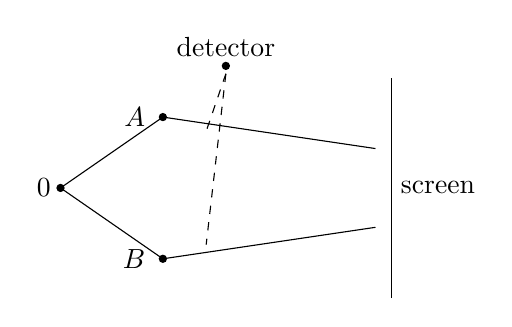
\begin{tikzpicture}[scale=1.0]
\fill (-2,0) circle (1.5pt);
\node[left] at (-2,0) {$0$};
\fill (-0.7,0.9) circle (1.5pt);
\node[left] at (-0.8,0.9) {$A$};
\fill (-0.7,-0.9) circle (1.5pt);
\node[left] at (-0.8,-0.9) {$B$};
\draw (-2,0) -- (-0.7,0.9);
\draw (-2,0) -- (-0.7,-0.9);
\draw (-0.7,0.9) -- (2.0,0.5);
\draw (-0.7,-0.9) -- (2.0,-0.5);
\draw (2.2,-1.4) -- (2.2,1.4);
\node[right] at (2.2,0) {screen};
\fill (0.1,1.55) circle (1.5pt);
\node[above] at (0.1,1.55) {detector};
\draw[dashed] (0.1,1.45) -- (-0.15,0.72);
\draw[dashed] (0.1,1.45) -- (-0.15,-0.72);
\end{tikzpicture}
\caption{対称な検出器配置の明快な再構成：両方の経路が同じ検出器状態を生み出す。}
\end{figure}

\begin{classroomqa}
\lecturetimestamp{00:27:55}
\audiencequestion{干渉が消える前に、誰かが実際に補助スピンを読まなければならないのか。}
\lecturerresponse{いいえ。電子はすでに自分の経路をスピンと相関させている。検出器をリセットし、一度に一電子ずつ実験を繰り返し、スクリーンへの衝突の分布だけを調べてもよい。誰もスピンを読まなくてもフリンジは現れない。重要なのは物理的な記録であり、それに対する人間の認識ではない。}
\end{classroomqa}

\begin{classroomqa}
\lecturetimestamp{00:29:36}
\audiencequestion{十分に軽い反跳する板は干渉を破壊するだろうか。}
\lecturerresponse{はい、反跳が二つの経路に対して板を直交する運動量状態へずらす場合には。ずれた波束が依然として重なるなら、破壊は部分的にとどまる。質量そのものが基準なのではなく、最終的な板の状態の区別可能性が基準である。}
\end{classroomqa}

放射はもう一つの不完全な記録装置を与える。加速された荷電粒子は光子を放出しうる。\(A\)の近くで放出された放射は、\(B\)の近くで放出された放射と同じ状態である必要はないので、電磁場は経路の情報を保持しうる。ゆっくり偏向される電子では、放出確率は小さくなりうる。講義では、およそ百回に一回という例示的な見積もりを用いている。より強い加速は放射を、したがってコントラストの損失をより起こりやすくする。重要な点は定性的である：観測されない光子でさえコヒーレンスを持ち去りうる。

\begin{classroomqa}
\lecturetimestamp{00:32:00}
\audiencequestion{不完全なコントラストをもつ実際の実験で、干渉確率をどのように推測するのか。}
\lecturerresponse{実験を何度も繰り返し、相対度数からスクリーン分布を推定する。有限のサンプルと環境の記録は、名目上暗い領域に残留カウントを残す。推測された確率分布は試行回数とともに改善する一方、デコヒーレンス過程は物理的なフリンジコントラストを減少させる。}
\end{classroomqa}

\begin{classroomqa}
\lecturetimestamp{00:33:13}
\audiencequestion{経路を決定する可能性は、すべての干渉を破壊するのだろうか。}
\lecturerresponse{完全な識別可能性は干渉を完全に破壊する。部分的な情報は部分的な損失をもたらす。わずかに回転するだけの検出器は2つの非直交な記録状態を残すので、検出器を読み取ると一方の経路が他方より確からしくなるが、確実ではない。それに対応して、縞は消去されるのではなくぼやける。}
\end{classroomqa}

\(|E_A\rangle\) と \(|E_B\rangle\) を任意の記録状態とする。スクリーンにおける合成状態は
\begin{equation}
|\Psi\rangle
=\sum_m\left(
\psi_m|m\rangle|E_A\rangle
+\phi_m|m\rangle|E_B\rangle
\right).
\end{equation}
と書ける。記録系を無視すると
\begin{align}
P(m)
&=|\psi_m|^2+|\phi_m|^2 \\
&\quad
+\psi_m^*\phi_m\langle E_A|E_B\rangle
+\phi_m^*\psi_m\langle E_B|E_A\rangle.
\end{align}
となる。したがって、重なり \(\langle E_A|E_B\rangle\) がコヒーレンス因子である。同一の記録は完全な干渉を保ち、直交する記録はそれを除去し、中間の重なりは中間の可視度を与える。

\begin{classroomqa}
\lecturetimestamp{00:34:12}
\audiencequestion{光子がときどきしか放出されない場合、光子放出事象のみを残すとどうなるか。}
\lecturerresponse{その選択された部分集団は一般に、光子が経路情報を運ぶため、より劣った干渉を示す。損失は完全である必要はない。2つの開口から放出された光子波束自体が重なりうるので、放射の記録でさえ完全に直交しないことがある。}
\end{classroomqa}

環境による衝撃はこの機構を拡大する。空気分子、周囲の光子、周囲の物質は、巨視的な位置の記録を絶えず獲得する。人や月は、可干渉な位置の重ね合わせに目に見えて広がったままではない。質量は自由な広がりを遅くし、絶え間ない環境とのもつれが、巨視的に分離した選択肢の間の観測可能な干渉を抑制する。

\begin{classroomqa}
\lecturetimestamp{00:36:02}
\audiencequestion{これはすでに測定の理論であり、単に \emph{波束の収縮} という語句の別の用法ではないのか。}
\lecturerresponse{これは、意図的に厳密な例における機構である。電子のみの記述では、収縮とは非対角項 \(\psi^*\phi\) を捨てることを意味する。合成系の記述では、場当たり的な削除は必要ない。直交する装置状態とのもつれが、それらの項を電子のみに対する測定には利用できないものにする。より複雑な例もこの構造にさかのぼって理解されるべきである。}
\end{classroomqa}

\begin{classroomqa}
\lecturetimestamp{00:38:04}
\audiencequestion{経路を曲げる重力場は、放射の議論や干渉の規則を自然に変えるのだろうか。}
\lecturerresponse{詳細な放射は変わりうるし、量子力学は経路測定の前に単一の鋭い軌道を割り当てない。一般的な結論は変わらない。識別可能な経路情報を保持する自由度だけが干渉を抑制する。より詳細な答えが意味を持つには、具体的な装置を指定しなければならない。}
\end{classroomqa}

\begin{classroomqa}
\lecturetimestamp{00:39:44}
\audiencequestion{この干渉は古典電磁波の干渉とは異なるのか。}
\lecturerresponse{多数の光子に対しては、観測されるパターンは電磁場の通常の波の干渉と一致する。単一粒子の実験は、より深い量子的な主張を示す。光子と電子は個々の事象として到着する一方、それらの量子振幅が干渉する。電子については、関連する波は電磁波ではなく電子の波動関数である。}
\end{classroomqa}

\begin{classroomqa}
\lecturetimestamp{00:40:45}
\audiencequestion{\(A\) と \(B\) の間に向けられた初期波の部分はどうなるのか。}
\lecturerresponse{この意図的に離散的な模型では、障壁の残りの部分は遮られている。それらの部分は反射され、透過したスクリーン振幅に寄与しない。この模型は、実際のビームが2つの運動量成分しか持たないと主張することなく、2つの透過した選択肢を分離する。}
\end{classroomqa}

\section{猫とスクリーンと可動な切断}

同じ数学が Schr\"odinger の猫にも当てはまる。銃が発射されていない状態と発射された状態に対して状態 \(|U\rangle\) と \(|F\rangle\) を持ち、猫が生きている状態と死んでいる状態に対して状態 \(|L\rangle\) と \(|D\rangle\) を持つとする。生きている猫と発射されていない銃から出発すると、相互作用は
\begin{equation}
|\Psi_{\mathrm{cat}}\rangle
=\alpha|L,U\rangle+\beta|D,F\rangle.
\end{equation}
を生じうる。猫だけはコヒーレント状態 \(\alpha|L\rangle+\beta|D\rangle\) にはない。それは選択肢を記録した銃ともつれている。銃を見れば猫の分岐が明らかになりうるし、直交する銃の記録は猫の部分系における通常の生--死の干渉を除去する。

\begin{classroomqa}
\lecturetimestamp{00:41:18}
\audiencequestion{猫自身は生きている状態と死んでいる状態の重ね合わせにあるのか。}
\lecturerresponse{単純に孤立した意味ではそうではない。複合系である猫と--銃の系は、相関した選択肢の重ね合わせにある。すなわち、生きていて銃が発射されていない場合と、死んでいて銃が発射された場合である。猫の部分系は記録を担う銃ともつれている。ちょうど電子の経路が補助スピンともつれているのとまったく同じである。}
\end{classroomqa}

最終スクリーンもまた装置として扱わなければならない。\(m\)に到達した電子は、写真乾板の粒子を黒くするか、シンチレータに光子を放出させるか、あるいは局所的な二状態素子の列の中の一つの検出器を反転させるかもしれない。その痕跡は到達位置と相関するようになる。

\begin{classroomqa}
\lecturetimestamp{00:43:38}
\audiencequestion{状態ベクトルだけで最後まで記述するのではなく、最終スクリーンでは確率について語ってよいのはなぜか。}
\lecturerresponse{確率の公準は、\(\langle\Pi_m\rangle\)を、\emph{到着位置が\(m\)}であるという性質に割り当てる。物理的な実験を完結させるために、スクリーンはその後、位置の記録を残す。射影演算子が確率を与え、黒化、シンチレーション、あるいは局所検出器の状態の反転が、統計の収集対象となる測定を実現する。}
\end{classroomqa}


\begin{classroomqa}
\lecturetimestamp{00:45:00}
\audiencequestion{なぜスクリーン測定について論じるのに、\(A\)や\(B\)を通る確率については論じないのか。}
\lecturerresponse{経路確率を割り当てて検証できるのは、経路記録装置を設置した場合だけである。そのような記録がなければ、選択肢はコヒーレントなままであり、振幅として加え合わされなければならない。スクリーンにおいては、位置に敏感な装置が仮定されている。この違いは特権的な時間ではなく、対応する測定相互作用が準備されているかどうかである。}
\end{classroomqa}

系と装置の境界は移動させることができる。記録状態\(|O_u\rangle\)と\(|O_d\rangle\)をもつ観測者を含めると、
\begin{equation}
|A,u\rangle+|B,d\rangle
\longrightarrow
|A,u,O_u\rangle+|B,d,O_d\rangle.
\end{equation}
別の観測者が今度は最初の観測者と相関するようになるかもしれない。猫の箱の中の煙、銃、猫、Schr\"odinger、そしてウィグナーはすべて、一つのより長いもつれの連鎖に含めることができる。境界をどこに引いても、相関は整合的であり続けなければならない。もしウィグナーが後にSchr\"odingerに自分が何を見たかを尋ねれば、彼らの記録は一致する。

\begin{classroomqa}
\lecturetimestamp{00:47:24}
\audiencequestion{系はどこで終わり、測定する観測者はどこから始まるべきなのか。}
\lecturerresponse{量子力学は唯一の都合のよい境界を選び出したりはしない。電子のみの記述を収縮させてもよいし、検出器を含めてより大きな記述を収縮させてもよいし、観測者を含めて再びもつれた状態を拡大してもよい。物理的要請は、アクセス可能なすべての確率と記録の整合性であって、唯一の帳簿上の境界ではない。}
\end{classroomqa}

\begin{classroomqa}
\lecturetimestamp{00:49:47}
\audiencequestion{経路を測定することが事象を乱すために不確定性原理が関与するのか。}
\lecturerresponse{はい。反跳の例はそのつながりを明示している。板の局在化は運動量の不確定性を生み、それが小さな経路依存のキックを識別可能にするのを妨げうる。より一般には、量子測定は系と--装置のもつれが状態を変化させるまで完結せず、その変化は後の干渉を変えうる。}
\end{classroomqa}

これは古典的理想との鋭い対照を際立たせる。古典的には、測定をいくらでも穏やかに行い、無視できるほどの擾乱で情報を引き出せると想像する。ここでは、経路情報を引き出すには装置との相関を確立することが必要である。それは結合状態の真の変化であり、後の干渉実験の答えを変える。

\begin{classroomqa}
\lecturetimestamp{00:52:06}
\audiencequestion{\(A\)と\(B\)の間の隔たりが非常に大きくなるとどうなるのか。}
\lecturerresponse{普遍的な新しい規則はない。この源と障壁の幾何学では、非常に遠くの開口に到達する振幅は単に小さくなるだけかもしれず、そのためほとんどの粒子は遮られた領域に当たる。\(\psi_m\)と\(\phi_m\)におけるこのような装置依存の変化を別にすれば、隔たりだけではコヒーレンスが生き残るかどうかを決めない。}
\end{classroomqa}

\begin{classroomqa}
\lecturetimestamp{00:53:04}
\audiencequestion{量子発展の線形性は根本的に厳密なのか、そしてなぜ自然はそれを用いるのか。}
\lecturerresponse{線形性は量子力学の経験的基礎である。小さな非線形修正は論理的に整合させるのが極めて困難であることで悪名高く、構造を損ないがちである。物理的命題が古典的集合ではなく部分空間の論理に従うという、より深い理由はここでは与えられない。講義はそれを自然の事実として扱う。}
\end{classroomqa}

\begin{classroomqa}
\lecturetimestamp{00:54:53}
\audiencequestion{後になってからの観測が、それ以前の経路を明らかにし、それによって干渉が起こったかどうかを変えうるだろうか？}
\lecturerresponse{後になってからの観測が経路を明らかにしうるなら、何らかの物理的自由度が経路に依存する記録を保存していなければならない。その記録はすでにコヒーレンスに影響を及ぼしている。誰かがそれを読む必要はない。因果性は依然として尊重されなければならず、抽象的な遅延選択の主張は、完全な時空配置と装置を指定することなしには決着をつけられない。}
\end{classroomqa}

\begin{classroomqa}
\lecturetimestamp{00:56:47}
\audiencequestion{開口部のすぐ後に泡箱を置いたらどうなるか？}
\lecturerresponse{二つの出てくる経路を区別する飛跡は曖昧さのない印であり、したがってそれらの干渉を破壊する。薄い経路記録層で十分である。下流の装置が、それ以前の開口部を推論するのに十分な情報を保持しないなら、それは自動的にどちらの経路かを見分ける検出器として働くわけではない。}
\end{classroomqa}

\begin{classroomqa}
\lecturetimestamp{00:59:29}
\audiencequestion{世界がすでに高度にもつれているなら、干渉実験はどうしてもつれていない系から始めることができるのか？}
\lecturerresponse{準備は、関連する自由度を、諸選択肢が同じ環境記録から始まるのに十分なほどに隔離し、リセットし、または条件づけなければならない。先行する泡箱の飛跡は、それが経路と相関したままであるなら、単に無視することはできない。干渉には、制御された系と関連する記録器との間の、積に近い初期関係が必要である。}
\end{classroomqa}

\begin{classroomqa}
\lecturetimestamp{01:01:04}
\audiencequestion{測定の後、実際的なもつれの解消はどこから来るのか？}
\lecturerresponse{確定した観測結果について条件づける。スピンが上向きに見出されたなら、観測者は分岐\(|A,u\rangle\)を保持し、代替の分岐を作業記述から捨てる。その条件付き積状態は新たな出発点として用いることができる。観測者を含めた完全な状態はもつれたままでありうるが、記録された結果に対しては、選択された準備は確定している。}
\end{classroomqa}

この入れ子状の階層はすべての解釈上の問いを解決するわけではないが、操作的整合性を可視化する。系、検出器、観測者、そして観測者の観測者までもがすべて含まれうる。記述をどこで切っても、正しく相関した記録は後になって互いに矛盾することはない。

\section{もつれからエントロピーへ}

議論は予定よりも測定の深みへと進んでしまったが、次の問いを明らかにした。すなわち、もつれの度合いはどのように測ることができるのか？　積状態にある二つのスピン
\begin{equation}
|u\rangle\otimes|u\rangle
\end{equation}
はもつれていない。各部分系はそれ自身の確定した状態をもち、一方を観測しても他方について新しい情報は得られない。もつれた状態はこのようには因数分解しない。標準的な定量的診断はもつれエントロピーとなるが、まず通常のエントロピーの概念、次にその量子形が必要である。

\section{欠けている情報としての古典エントロピー}

\(N\)個の可能な状態をもつ古典系から始める。ここでのエントロピーは、系とそれについての我々の知識とを合わせた性質である。我々が知っているのが、系が等確率の\(n\)個の状態のうちの一つを占めるということだけであるとしよう。そのとき
\begin{equation}
S=\log n.
\end{equation}
である。\(n=1\)なら状態は既知であり\(S=0\)である。\(n=N\)なら、状態空間そのもの以外には何も知られておらず、エントロピーは最大で\(S_{\max}=\log N\)である。

対数は独立なはい--いいえの選択を加法的に数える。\(M\)個の古典スピンに対しては\(2^M\)個の配置があるので、
\begin{equation}
\log(2^M)=M\log 2.
\end{equation}
である。したがって、対数の底の選択を除いて、エントロピーは記述から欠けている二進情報の量を数えている。

一般の確率分布\(p_i\)に対して、適切な定義は
\begin{equation}
S=-\sum_i p_i\log p_i.
\end{equation}
である。

\begin{classroomqa}
\lecturetimestamp{01:14:17}
\audiencequestion{なぜエントロピーの式には負号があるのか？}
\lecturerresponse{すべての非零の確率は\(0<p_i\leq 1\)を満たすので、\(\log p_i\leq 0\)である。負号はエントロピーを非負にする。\(p_i=0\)では、寄与は極限\(p_i\log p_i\to0\)によって定義される。}
\end{classroomqa}

等確率分布
\begin{equation}
p_i=
\begin{cases}
1/n, & i\in\mathcal N,\\
0, & i\notin\mathcal N,
\end{cases}
\qquad |\mathcal N|=n,
\end{equation}
に対して、一般式は
\begin{align}
S
&=-n\left(\frac1n\right)\log\left(\frac1n\right)\\
&=\log n.
\end{align}
となる。したがってそれは初等的な数え上げの定義を再現する。一つの状態に確実に集中した分布は\(S=0\)をもつ。

\begin{figure}[htbp]
\centering
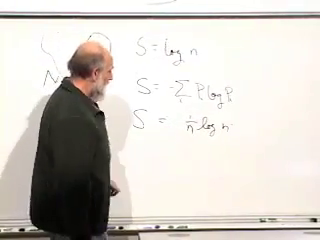
\includegraphics[width=0.66\textwidth]{lecture_07_figure_07.png}
\caption{板書は\(S=\log n\)、シャノンの式、および等確率の確認をまとめている。}
\lectureframe{01:16:08}
\end{figure}

\begin{classroomqa}
\lecturetimestamp{01:17:35}
\audiencequestion{\(N\)個の状態をもつ系が持ちうる最大のエントロピーは何であり、その場合には何が分かっているのか。}
\lecturerresponse{最大値は\(\log N\)であり、一様分布\(p_i=1/N\)によって達成される。その場合でも系が何であるかは依然として分かっており、したがってその状態空間も分かっている。分かっていないのは、その\(N\)個の状態のうちどれを占めているかである。}
\end{classroomqa}

差
\begin{equation}
I=S_{\max}-S
\end{equation}
は、この数え上げの意味での利用可能な情報である。エントロピーと情報は同じ記帳の裏表である。エントロピーは、状態を区別しうるが我々には利用できない情報を記録している。

\section{トレース：和に対する量子的な置き換え}

演算子\(M\)と任意の完全正規直交基底\(\{|i\rangle\}\)に対し、
\begin{equation}
\operatorname{Tr}M
=\sum_i\langle i|M|i\rangle.
\end{equation}
と定義する。

\begin{figure}[htbp]
\centering
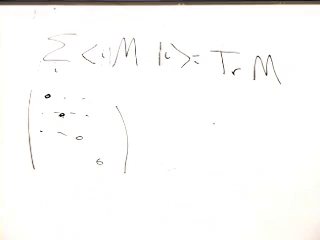
\includegraphics[width=0.68\textwidth]{lecture_07_figure_08.png}
\caption{対角行列要素の和として書かれたトレース。}
\lectureframe{01:21:20}
\end{figure}

定義は基底を用いて書かれているが、結果は基底に依存しない。エルミート演算子に対しては固有基底を選ぶことができ、そのとき
\begin{equation}
\operatorname{Tr}M=\sum_i\lambda_i.
\end{equation}
固有値、したがってその和は、演算子を表すのに用いた座標に依存しない。

\begin{classroomqa}
\lecturetimestamp{01:23:04}
\audiencequestion{行列を対角形にすることは、それが逆行列をもつことを意味するのか。}
\lecturerresponse{いいえ。対角形は固有値を示すものであり、可逆性は別個の条件である。対角行列が可逆であるのは、その対角固有値のどれもゼロでないとき、まさにそのときに限る。エルミート行列は、いくつかの固有値が消える場合でも対角化可能である。}
\end{classroomqa}

休憩の後、古典確率に少し戻る。古典的可観測量は配位の関数\(f_i\)であり、その平均は
\begin{equation}
\langle f\rangle_{\mathrm{cl}}=\sum_i p_i f_i.
\end{equation}
である。量子論の公式では、トレースが選択肢にわたる和を置き換え、演算子が古典的関数を置き換え、密度行列が確率分布を置き換えることになる。

\section{統計的混合と密度行列}

誰かが系を正規直交基底のある状態に準備したが、どの状態が選ばれたかを我々に告げないとしよう。その人は準備確率だけを与える---例えば、スピンが確率\(3/4\)で上、確率\(1/4\)で下に準備される。これはコヒーレントな重ね合わせ
\begin{equation}
\sqrt{\frac34}|u\rangle+\sqrt{\frac14}|d\rangle,
\end{equation}
ではない。なぜなら相対位相は準備されていないからである。これは確定した状態の統計的混合である。純粋状態が分かっている場合でも量子確率は残る。ここでは、どの純粋状態が準備されたかについて追加の不確かさがある。

\begin{figure}[htbp]
\centering
\includegraphics[width=0.66\textwidth]{lecture_07_figure_06.png}
\caption{指定されたケットからアンサンブル記述への概念的移行。}
\lectureframe{01:29:43}
\end{figure}

状態\(|i\rangle\)が確率\(\rho_i\)で準備されるなら、密度演算子は
\begin{equation}
\rho=\sum_i\rho_i|i\rangle\langle i|.
\end{equation}
であり、準備基底では
\begin{equation}
\rho=
\begin{pmatrix}
\rho_1&0&0&\cdots\\
0&\rho_2&0&\cdots\\
0&0&\rho_3&\cdots\\
\vdots&\vdots&\vdots&\ddots
\end{pmatrix}.
\end{equation}
となる。

\begin{figure}[htbp]
\centering
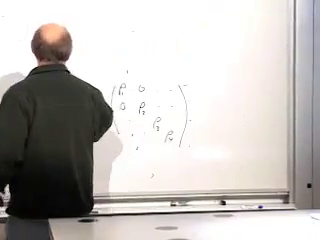
\includegraphics[width=0.68\textwidth]{lecture_07_figure_09.png}
\caption{対角密度行列とその規格化条件。}
\lectureframe{01:32:12}
\end{figure}

その固有値は実で非負であり、確率の規格化は
\begin{equation}
\operatorname{Tr}\rho=\sum_i\rho_i=1.
\end{equation}
となる。

\(F\)をエルミート可観測量とする。アンサンブル期待値は
\begin{equation}
\langle F\rangle=\operatorname{Tr}(F\rho).
\end{equation}
である。

\begin{figure}[htbp]
\centering
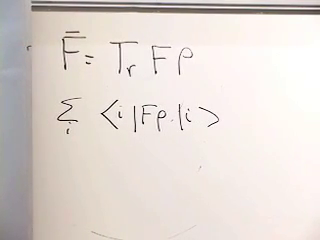
\includegraphics[width=0.68\textwidth]{lecture_07_figure_10.png}
\caption{トレース期待値\(\langle F\rangle=\operatorname{Tr}(F\rho)\)。}
\lectureframe{01:35:05}
\end{figure}

通常の重み付き平均を回復するには、\(\rho\)が対角となる基底でトレースを評価し、恒等演算子の分解を挿入すればよい：
\begin{align}
\operatorname{Tr}(F\rho)
&=\sum_i\langle i|F\rho|i\rangle\\
&=\sum_{i,j}\langle i|F|j\rangle
               \langle j|\rho|i\rangle\\
&=\sum_i\rho_i\langle i|F|i\rangle.
\end{align}
したがって、各純粋状態の期待値は、対応する状態が準備された確率で重み付けられる。

トレースは巡回性
\begin{equation}
\operatorname{Tr}(AB)=\operatorname{Tr}(BA),
\end{equation}
をもつ。\(A\)と\(B\)が可換でない場合でも成り立つ。したがって\(\operatorname{Tr}(F\rho)=\operatorname{Tr}(\rho F)\)である。

\section{量子エントロピーと先延ばしにされた報酬}

密度行列のエントロピーは
\begin{equation}
S(\rho)=-\operatorname{Tr}(\rho\log\rho).
\end{equation}
である。エルミート正演算子に対しては、\(\log\rho\)のような関数はその固有値を通じて定義される。もし
\begin{equation}
\rho=\sum_i\rho_i|i\rangle\langle i|,
\end{equation}
ならば
\begin{equation}
\log\rho=\sum_{\rho_i>0}(\log\rho_i)|i\rangle\langle i|,
\end{equation}
であり、したがって
\begin{equation}
S(\rho)=-\sum_i\rho_i\log\rho_i.
\end{equation}
となる。

\begin{figure}[htbp]
\centering
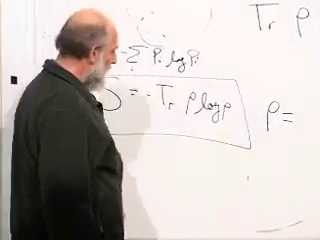
\includegraphics[width=0.68\textwidth]{lecture_07_figure_11.png}
\caption{古典的エントロピーの公式を\(S=-\operatorname{Tr}(\rho\log\rho)\)として書き直したもの。}
\lectureframe{01:41:25}
\end{figure}

既知の純粋状態は密度演算子
\begin{equation}
\rho_\psi=|\psi\rangle\langle\psi|,
\end{equation}
をもち、固有値は\(1,0,\ldots\)であるから、\(S(\rho_\psi)=0\)である。これは、\(|\psi\rangle\)に対するあらゆる測定が確定した結果をもつという意味ではない。準備された状態について追加の統計的無知がないという意味である。反対の極端では、
\begin{equation}
\rho=\frac{I}{d}
\qquad\Longrightarrow\qquad
S(\rho)=\log d,
\end{equation}
であり、ここで\(d=\dim\mathcal H\)である。最大混合状態は、あらゆる直交方向に等しい重みを割り当てる。

もつれとの関連は今や近いが、まだ解明されていない。合成系\(AB\)が結合状態にあり、すべての実験が\(A\)に限定されているとしよう。\(B\)を無視しつつ\(A\)上で得られるあらゆる期待値を再現する対象が存在しなければならない。その対象は\(A\)の密度行列である。結合状態が因数分解するならば、\(A\)の密度行列は純粋であり、エントロピーはゼロである。\(A\)と\(B\)がもつれているならば、\(A\)の密度行列は一般に混合であり、エントロピーは非ゼロである。その縮約密度行列を構成し、そのエントロピーを評価することが、次の講義に残された課題である。
